\documentclass[../main.tex]{subfiles}
%=========================================
%               Appendices
% =========================================
\begin{document}

\counterwithin{figure}{section} % Figures counters reinitialised
\newpage
\appendixpage
\begin{appendix}
    \section{Logbook}
    \subsection{Iteration from Monday 4th May to Friday 15th May}
    \paragraph{Objectives of the iteration :} 
    The main goal of this iteration was to get more familiar with WinCC-OA and the JCOP Framework. 
    Also the main idea was to think about how to make the LHCb experiments monitor more accessible from the web without changing the WinCC-OA pre-existing project drastically.
    \paragraph{Tasks done \& notes :}
    \begin{itemize}
        \item Reading documentations about WinCC-OA.
        \item Setting up the main project.
        \item Reading/Writting emails to the ISIMA supervisor (Mr HILL) and the CERN one (Mr Luis Granado Cardoso).
        \item Helping and exchanging with Loann, who is working on the same technology as me.
        \item Going through the tutorial slides.
        \item Experimenting through Exercice 1,2,3 and 4.
        \item Facing some difficulties with the CTRL system.
        \item Reading documentation about HttpServer
        \item Watching videos about WinCC-OA on \href{https://www.youtube.com/user/ETM2011}{Siemens} and \href{https://www.youtube.com/channel/UCGBnHd1-B-Zg9MDsjTk0-Sw}{KAASM}'s youtube channel. 
        \item Doing daily meetings with Luis to track the progess.
    \end{itemize}

    \subsection{Iteration from Wednesday 15th May to Sunday 20th May}
    \paragraph{Objectives of the iteration :}
    The aim of this iteration was to look at all the documentation about the WebServer components in WinCC-OA, how to navigate properly between panels, how to manage users access permissions and restrictions, and how to well organise configs files in a project. I was sick during a part of this iteration, so I did not work effictively on Monday
    \paragraph{Task done :}
    \begin{itemize}
        \item Reading all the documentation
    \end{itemize}

    \paragraph{Notes :} 
    I have been reading the documentation about the configuration files :
    \begin{itemize}
        \item config.level is for managers configurations, and basically, loading libs through this file.
        \item config.redu is for redundancy, that we are not seeking for, at the moment
        \item config.http is a premade file from the WinCC-OA folder
        \item config.webclient is an additional file for configuration Desktop and Mobile UI add-ons\dots (Not what we are looking for)
    \end{itemize}
    I have tested multiple stuffs on those. Nothing really can simplify the actual config (root) file.
    I guess there's another option not yet tested which is the own configuration file, I don't know if we can use more than once.\newline
    For the navigation fluidify and simplification issues, I have been testing stuffs and reading about the differences between Modules, Embedded Modules , Child and Root Panel.\newline
    To navigate properly, I think I should take a look at the Topologies panels components... The embedded modules through one root module, may be the best layout option.

    \subsection{Iteration from Wednesday 20th May to Wednesday 27th May}
    \paragraph{Objectives of the iteration :}
    \begin{itemize}
        \item User permissions, one can connect to view, another can connect to administrate
        \item Play with the alarm Screen, make a shortcut to it
        \item (FSM) Implement one, how it goes on the ULC components
    \end{itemize}
    \paragraph{Tasks done :}
    \begin{itemize}
        \item Login panel has been implemented (worked on both ULC and Regular WinCC)
        \item Can access on user admnistration panel through it : Module \textgreater\ SysMgm \textgreater\ Permissions \textgreater\ User Admnistration, which on root access list all users and permissions
        \item Groups \textgreater\ Admnistrate \textgreater\ Permissions : You can change the group permissions but also, create new groups with new permissions
        \item Permissions are logged in an Authorization Bits system. The first five bits are already define, they are predefined and un-changeable, but you can change the description if you want and texts of it : 
        \begin{itemize}
            \item 1 : Visualisation: Visualize only
            \item 2 : Normal operator authorization: permits the opening of child panels.
            \item 3 : Advanced operator authorization: permits execution of commands, explicit setting of replacement values, input of correction values as well as changes to all value range types.
            \item 4 : Administration: permits the use of the PARA.
            \item 5 : Acknowledgement: permits acknowledgment of alerts.
            \item 32 : Allows SSO for one work station
        \end{itemize}
        \item Can also access on login statistics panel to see whose connected : Module \textgreater\  Login Statistics
        \item We can manage the Components access thanks to the boolean getUserPermission() function : CONTROL \textgreater\  Control functions \textgreater\ G \textgreater\ getUserPermission()
        \item We can check on the Main Panel, by Login via Guest or via Root
        \item Auto login done, with inactivity (Glitch with inactivity, security one) (UI number changed some time)
        \item Alarm Panel : I have worked on it, but there is a glitchy features, the windows appears behind the Alarm Screen
        \item I also haven't the time to experiment on the FSM.
    \end{itemize}

    \subsection{Iteration from Wednesday 27th May to Tuesday 2nd June}
    \paragraph{Objectives of the iteration :}
    \begin{itemize}
        \item Adding and testing the FSM, on the Web app, it actually works but... it took me a lot of times.
        \item Create Shortcut for opening differents kinds of panels, I had issues with the DEN Panel... But now it works
        \item Didn't check on the Alarm Screen and the Users Permissions, as I had issues with the DNS part of the tuturials.
    \end{itemize}

    \subsection{Iteration from Thurday 3rd June to Monday 8th June}
    \paragraph{Objectives of the iteration :}
    \begin{itemize}
        \item Look at the documentation about Distribution Manager, Distribution Configs Files, Distributions Systems etc...
        \item Test to implement the following panel : \\ (Location : /localdisk/wincc/prod/["LBECSINFO","ECS"]/panels/)
        \begin{itemize}
            \item lbAlarmHandling/lbAlarmScreen.pnl
            \item FarmUsagePlot.pnl
            \item lbECS/lbOPCMonitor.pnl
            \item lbTriggers/lbTriggersOverview.pnl
            \item lbTrending/lbTrending.pnl
        \end{itemize}
        \item Use the current project as the main client, connected to the ECS and LBECSINFO projects.
    \end{itemize}
    I have read a lot of the documentation about the distributed managements, and distributed systems.
    I have learnt that you can configure them through an existing wizard only if you create a new project.
    Else you should do it via the configuration files. I have tried to launch script from the copied project, but without any success. \newline
    The Test Project configuration file should look like this :\newline
    [general]\newline
    distributed = 1\newline
    [dist]\newline
    distPeer = "dist\_name\_ECS" 1130\newline
    distPeer = "dist\_name\_LBECSINFO" 1140

    \begin{figure}[h]
        \centering
        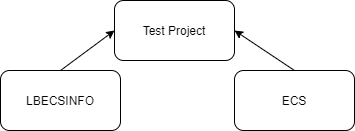
\includegraphics[scale = 0.5]{images/subsystem.png}
        \caption{Example of distributed projetcs}
    \end{figure}

    \subsection{Iteration from Monday 8th June to Wednesday 10th June}
    \paragraph{Objectives of the iteration :}
    The meeting with Luis helped me debugging the and connecting the two distributed projects. I am currently trying to launch differents panels from the ULC web components.
    I have succeed to open them, but... the data point seems to not be well-connected or at least are connected to the wrong project.
    I achieved this by updating the config files, which is I think not the cleanest way to do it, but the fastest (Testing first)
    We can explore two options which are : copying all the project in a special repos, or we can try with the addSymbol() functions, or we can also try to copy all the paths.

    \subsection{Iteration from Friday 12th June to Friday 19th June}
    \paragraph{Objectives of the iteration :}
    Connect all those panels and see if they work properly in the ULC UX components. See panels from iteration 03/06 to 08/06
    \subsection{Iteration from Friday 19th June to Wednesday 24th June}
    \paragraph{Objectives of this iteration :}
    \begin{itemize}
        \item Create a new main page for the app, which should be more similar than the one already in use.
        \item Create shortcuts to the following panels :
        \begin{itemize}
            \item LHCb Top FSM - Without the possibility to click anywhere
            \item LHCb - LHC - Big Brother
            \item Alarms Screen
            \item Trending panels
        \end{itemize}
        \item Also check if we can have to access to other stuffs than WinCC-OA panels onto the ULC UX components.
    \end{itemize}
    \paragraph{Notes :}
    I have issues on displaying both FSM from ECS. Seems that there are missing datapoints. Also, I have noticed some stuffs on the right click event.
    I need to go deep down the code of the Alarm Panel and the Trending one, too see why it's working only if you launch the Alarm panel before.
    I also need to continue on the tools bars.
    \subsection{Iteration from Wednesday 24th June to Tuesday 30th June}
    \paragraph{Objectives of this iteration :}
    \begin{itemize}
        \item Continue the investigation and research on the IFrame stuffs.
        \item See if we can fix the right-click issues as I have new hints.
        \item Wait until Luis fix the DP non-exists from the LHCb Top \& BigBrother panels.
        \item Also continue with the tools bars customizations.
    \end{itemize}
    \paragraph{Notes :}
    \paragraph{Investigates :}
    \begin{itemize}
        \item navigation buttons, layout managements
        \item tabs for the layout
    \end{itemize}
    \subsection{Iteration from Tuesday 30th June to Monday 6th June}
    \subsection{Iteration from Monday 6th July to Monday 13th July}
    \subsection{Iteration from Monday 13th July to Wednesday 15th July}
    \subsection{Iteration from Wednesday 15th July to Friday 17th July}
    \subsection{Iteration from Friday 17th July to Tuesday 21st July}
    \subsection{Iteration from Tuesday 21st July to Friday 24th July}
    \subsection{Iteration from Friday 24th to Friday 31st July}

    
    For next Thursday 11hOO : 
    - Send HILL contact to Luis - (DONE)
    - LHCb Top / Big Brother to display correctly through personal panel : FSM ui panel
    - FarmUsagePlot -> Luis will use another plot (DONE)
    - Figure out the right click issues on the Trending pnl
    - Polish the look of the panels (DONE)
    - Layout for the WebViewer make this resizeable (DONE)
    - Make button directly goes to the part of web logbook (DONE)

    4 o'clock at the afternoon
    dummy data for tomorrow
    fsm thingy
    to prove that it can be used, and easy way to access the data, to be able to extend
    \newpage
    \section{Real Gantt chart}
    \begin{figure}[h]
        \centering
        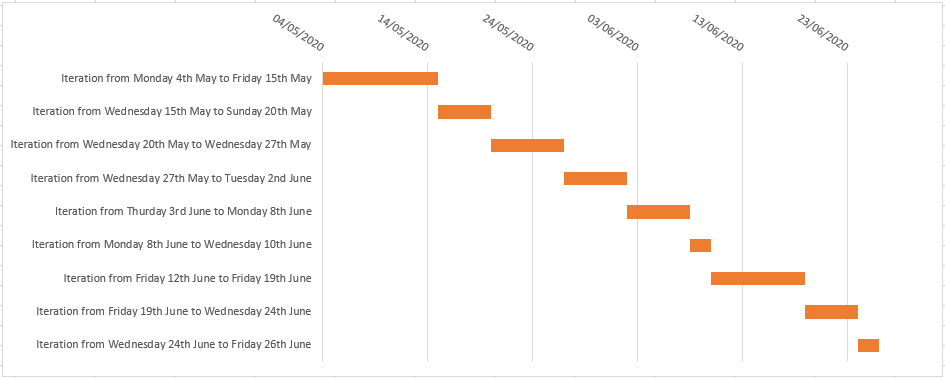
\includegraphics[scale = 0.6]{images/gantt.png}
        \caption{Real Gantt Chart}
    \end{figure}
\end{appendix}

\end{document}